\newpage
\section{Training our own models.} \label{training}

In this section we will present out results with training our own models. We will start by presenting the data sets used and then go on to present the reults of running the  PCA, VAE and DCGAN models on the data.

\subsection{Data sets}
In the following we will use two different datasets which we will refer to as the \emph{Caltech} and teh  \emph{FFHQ} dataset respectively. 1)  \emph{Caltech} \footnote{Available at \url{http://www.vision.caltech.edu/html-files/archive.html}} which consists of "450 frontal face images of 27 or so unique people." and 2) \emph{FFHQ}\footnote{Available at \url{https://github.com/NVlabs/ffhq-dataset}} Here we use the 5000 of the provided thumbnails of resolution 128x128.

The FFHQ dataset is already preprocessed such that the faces are aligned and the images are of the same dimensions. For Caltech however we need to do this preprocessing manually.

In the Github repository for this project we provide code to download both datasets with additional preprocessing  (face extraction and resizing to 128x128) of the Caltech dataset.\footnote{Code is available here: \url{https://github.com/renhaa/faces/blob/master/DownloadDataset.ipynb}}

In Figure \ref{rawdata} we see a random sample of the processed images from the Caltech \ref{raw-caltech} and FFHQ \ref{raw-ffhq} datasets respectively.

\begin{figure}[h!]
    \centering
    \begin{subfigure}[b]{0.45\textwidth}
        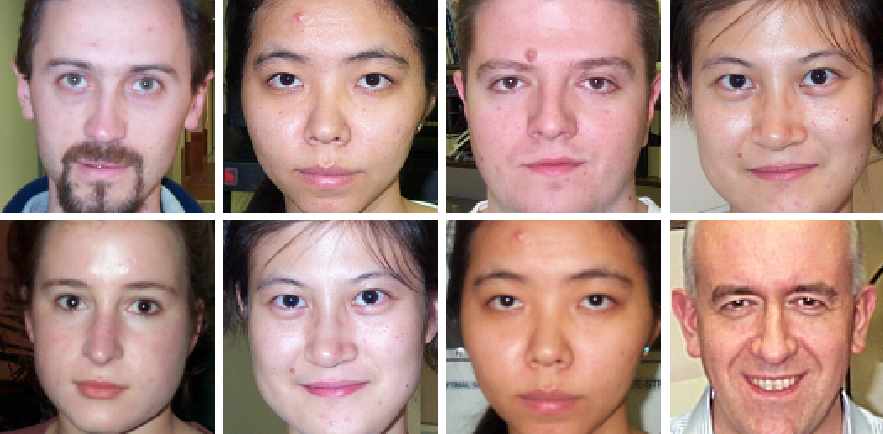
\includegraphics[width=\textwidth]{fig/data/caltech}
        \caption{Caltech dataset}
        \label{raw-caltech}
    \end{subfigure}
    ~
    \begin{subfigure}[b]{0.45\textwidth}
        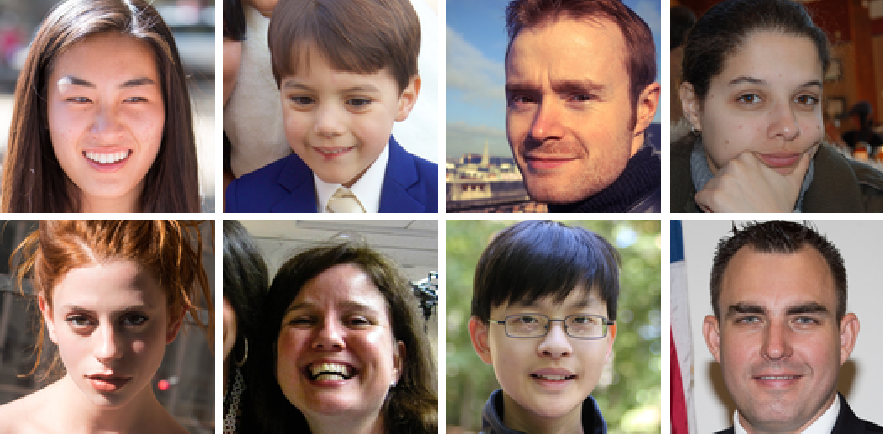
\includegraphics[width=\textwidth]{fig/data/ffhq}
        \caption{FFHQ dataset}
        \label{raw-ffhq}
    \end{subfigure}

    \caption{The raw data from the Caltech and FFHQ datasets respectively.}
    \label{rawdata}
\end{figure}

The FFHQ dataset have a much higher variation than the Caltech dataset, having samples of faces across all ages poses and ethnicity which the Caltech dataset is more limited having the same 27 people facing directly at the camera. 

In the following we will use both the colored version of the datasets and for some models we will use a black and white version. 

\subsection{Principal Component Analysis}

Here we present our results of doing Proncipal Component analasis on the FFHQ dataset. 

In the process of constructing the design matrix we simply flatten ech of the 120x120x3 dimensional color images to 49152 dimensional flat vectors. The normalize these vectors to zero mean and unit variance using\\ {\tt sklearn.preprocessing.StandardScaler} and calulate the eigenfaces with {\tt sklearn.decomposition.PCA}\footnote{The code is available here: \url{https://github.com/renhaa/faces/blob/master/PCA.ipynb}}

In Figure \ref{eigenfacehere} we see the first 8 eigenfaces. In Figure. \ref{eigenface} in the appendix there is a larger version of this figure. We note that the generated faces from the caltech dataset have some artefacts in the form of shadowy lines across the faces. This are not present in the faces generated from training on the FFHQ dataset, these imates are however slightly blurry.   

In Figure \ref{components} we see the result of adding or subtracting the 4th 5th and 6th eigenface to the mean face according to eq.\ref{eigenface-interpolate}. A larger figure showing this for the first six principal components can be seen in Figure \ref{pca-components} in the appendix. 

We see that the PCA algorithms is able we capture meaningful aspect of the dataset.
By visual inspection we observe that it seems that the first two Principal Components control aspects of color and ligthing, the third compoent controls the direction of lighting (is the lighting is from the left or the right). The fourth principal component seems to control ligthing from top to bottom but it could also seem like this component captures age. The fifth component clearly controls pose while the sixth component seems to be related to gender.

\begin{figure} [h!]
\centering
    \begin{subfigure}[b]{0.55\textwidth}
    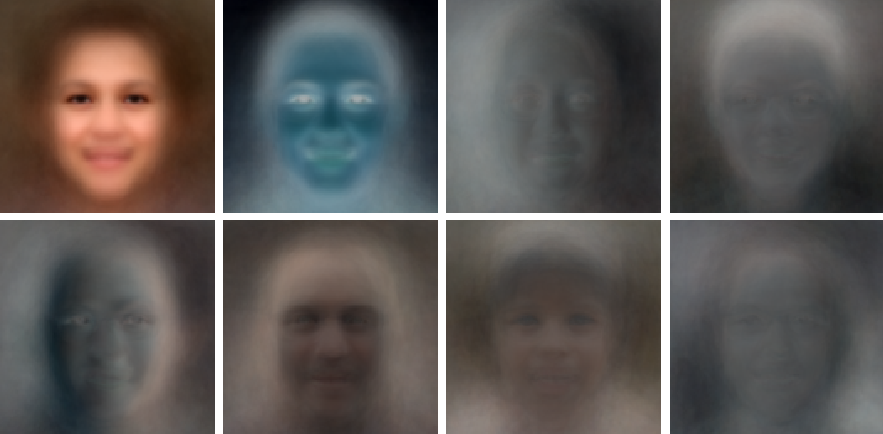
\includegraphics[height=3.2cm]{fig/PCA/pca}
     \caption{The first 8 eigenfaces from the FFHQ dataset.}
    \label{eigenfacehere}
    \end{subfigure}
    ~
    \begin{subfigure}[b]{0.4\textwidth}
        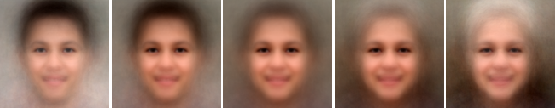
\includegraphics[height=1cm]{fig/PCA/pca3}
        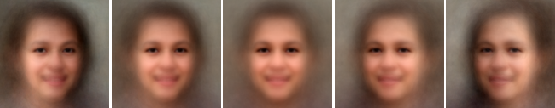
\includegraphics[height=1cm]{fig/PCA/pca4}
         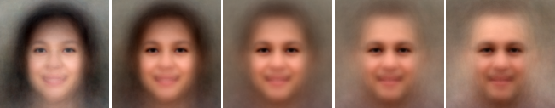
\includegraphics[height=1cm]{fig/PCA/pca5}
         \caption{Mean face shifted by the 4-6th eigenface.}
         \label{components}
    \end{subfigure}
     \caption{ In Figure. \ref{eigenfacehere} we see the Eigenfaces of the FFHQ dataset while in Figure. \ref{components} we see the mean face edited by by adding or subtracting the 4-6th eigenface from the mean face according to eq.\ref{eigenface-interpolate}.}
\end{figure}
Although Principal Component Analasis enables us to generate new faces and manipulate different aspects of the synthesized faces the results are still blurry, and nowhere near as photorealistic as the faces we will be able to generate with a pretrained Genrative Adversarial Network in Section \ref{stylegan}.

\subsection{VAE}
To train a Variational Autoencoder we use a modified version of the VAE implementation from the keras documentation \footnote{ Available here: \url{https://keras.io/examples/variational_autoencoder/}}. In the implementation the encoder and decoder are both modelled by multilayer perceptrons. We sse a latent space dimensition of 100 which is the same as for the DCGAN model which we present in the next subsection.   

In Figure \ref{vaeresults} we see the result of training the VAE for 4000 epochs on a black and white version of the datasets. We choose to train for 4000 epochs as this is about the maximum durations which was possible to train in google colab before the runtime was reset. The training time for the FFHQ dataset was about 7-8 hours. We make the Jupyter notebook which generate these images available with this project.\footnote{Available here: \url{ https://github.com/renhaa/faces/blob/master/VAE.ipynb}}

\begin{figure}[h!]
\centering
\begin{subfigure}[b]{0.45\textwidth}
     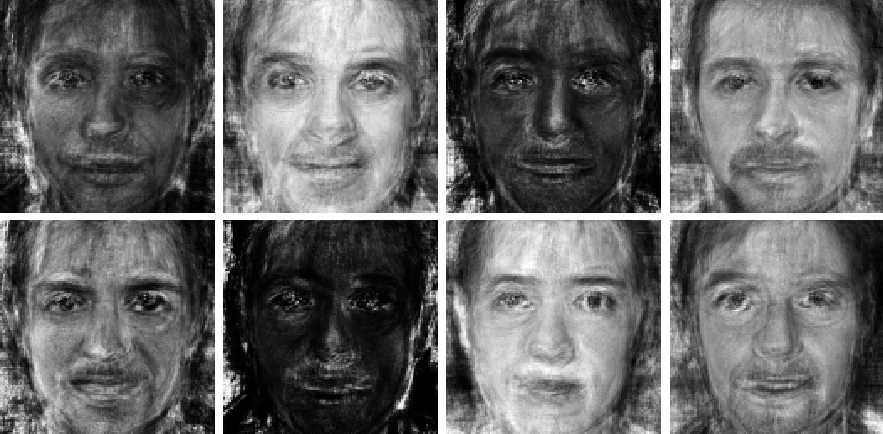
\includegraphics[width=\textwidth]{fig/vae/caltech_epoch4000}
    \caption{caltech}
\end{subfigure}
    ~
\begin{subfigure}[b]{0.45\textwidth}
     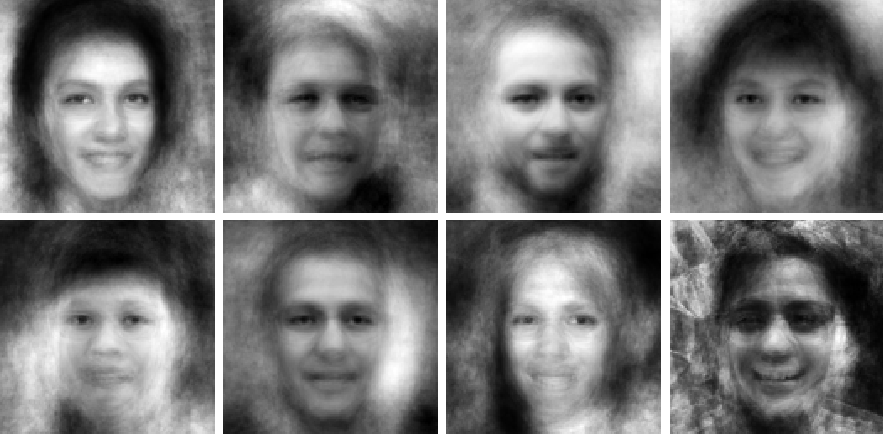
\includegraphics[width=\textwidth]{fig/vae/ffhq_epoch4000}
    \caption{ffhq}
\end{subfigure}
\caption{Samples from Variational Autoencoder during training on a black and white version of the Caltech and FFHQ dataset}
\label{vaeresults}
\end{figure}

Larger figures with samples drawn during traing can be seen in Figure \ref{vaq-bwffhq-samples} and Figure \ref{vaq-bwcaltech-samples}. 

We also tried to train the VAE on color images but the results were unstable. The images during training can be seen in Figure \ref{vaq-ffhq-samples}. As can bee seen in the figure it seems that the model was improving at least until epoch 2000. But then at epoch 4000 the network suddenly did not improve anymore and there was little variation in the generated samlples. This problem also happened for the Caltech dataset. 



\subsection{DCGAN}
In this section we will present our results with training a Deep Convolutional Generative Adversarial Network (DCGAN). \footnote{Concretely we use modified version of from \url{https://github.com/eriklindernoren/Keras-GAN/blob/master/dcgan/dcgan.py}} \footnote{The nodebook generating the results presented here can be found at: \url{https://github.com/renhaa/faces/blob/master/DCGAN.ipynb}}

The models uses four convolutional layers in with the generator and discriminator and the implenmentation follows the guidelines presented in \cite{dcgan} where we use strided convolutions, batchnormalization and Leaky ReLU in the discrimintaro while the generator uses normal ReLU in all hidden layers exept the last where we use the hyperbolic tangent.In figure \ref{dcgan-results} we see the results from training a DCGAN the FFHQ and Caltech datasets for 10000 epochs. The training time was about 9-10 hours  using Google Colab.

\begin{figure}[h!]
    \centering
    \begin{subfigure}[b]{0.45\textwidth}
        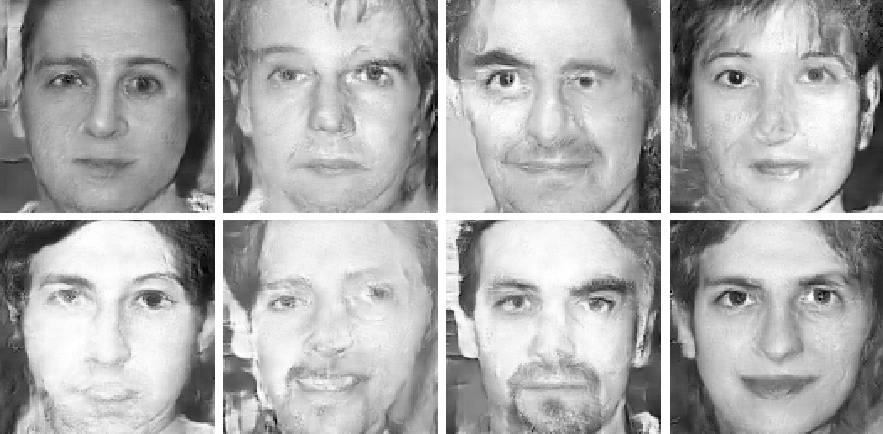
\includegraphics[width=\textwidth]{fig/dcgan/caltech/epoch10000}
        \caption{Caltech dataset B/W}
        \label{dcgan-caltech}
    \end{subfigure}
    ~
    \begin{subfigure}[b]{0.45\textwidth}
        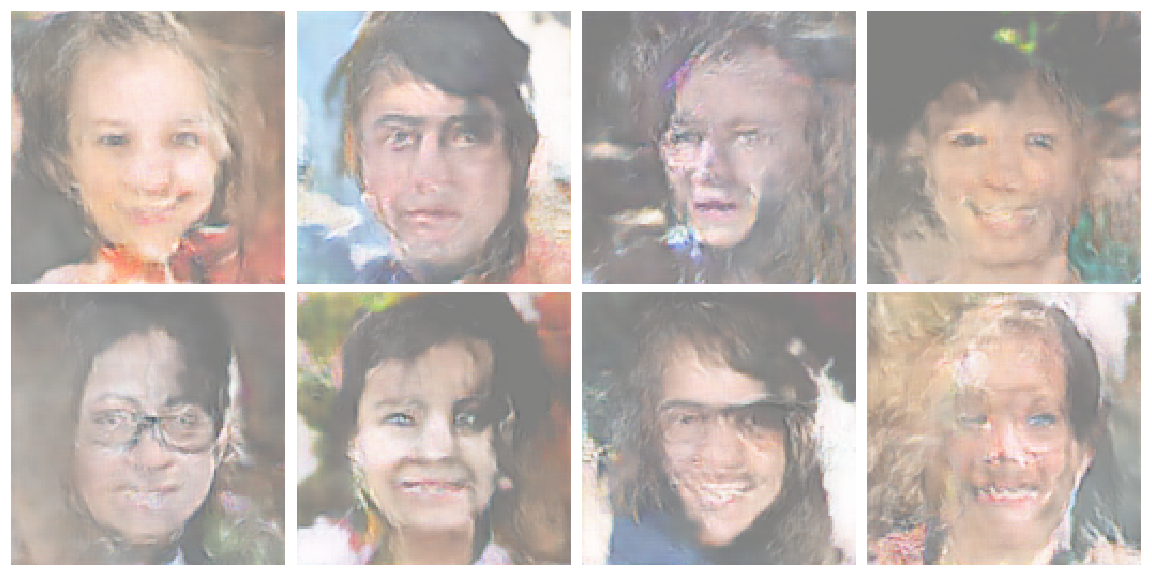
\includegraphics[width=\textwidth]{fig/dcgan/ffhq/epoch10000}
        \caption{FFHQ dataset}
        \label{dcgan-ffhq}
    \end{subfigure}
    \caption{The results from training the DCGAN for 10000 epochs on the FFHQ and Caltech datasets respectively.}
    \label{dcgan-results}
\end{figure}

We see that this model is able to produce relatively decent images on the black and white version of the caltech dataset (Figure \ref{dcgan-caltech}). Sometimes we generate an image which could be mistaken for being real. Upon further imspection howefter, we note that the generated images are always somewhat similar to one of the 27 persons in the dataset. Thus it seem that we are able to create better quality images but with lower variation using the Caltech dataset compared to the FFHQ dataset. We argue that the generated images procudes here by DCGAN are of better quality and than the corresponding images synthesized by the Variational Autoencoder in the previous subsection. 

The generated images by training the DCGAn on the FFHQ are however, as we see in Figure \ref{dcgan-ffhq}, no where near photorealism. 
